\documentclass{beamer}
\usepackage{beamerthemesplit}
\usetheme{SPbGU}
%{CambridgeUS}
% Выпишем часть возможных стилей, некоторые из них могут содержать
% дополнительные опции
% Darmstadt, Ilmenau, CambridgeUS, default, Bergen, Madrid, AnnArbor,Pittsburg, Rochester,
% Antiles, Montpellier, Berkley, Berlin
\usepackage{pdfpages}
\usepackage{amsmath}
\usepackage{cmap} % for serchable pdf's
\usepackage[T2A]{fontenc} 
\usepackage[utf8]{inputenc}
\usepackage[english,russian]{babel}
\usepackage{indentfirst}
\usepackage{amsmath}
\usepackage{dot2texi}
\usepackage{tikz}
\usepackage{graphicx}
\usetikzlibrary{shapes,arrows}
% Если у вас есть логотип вашей кафедры, факультета или университета, то
% его можно включить в презентацию.

%\usefoottemplate{\vbox{}}%  \tinycolouredline{structure!25}% {\color{white}\textbf{\insertshortauthor\hfill% \insertshortinstitute}}% \tinycolouredline{structure}% {\color{white}\textbf{\insertshorttitle}\hfill}% }}

%\logo{
\includegraphics[width=1cm]{SPbGU_Logo.png}}

%[GLR-анализатор]
\title[YaccConstructor]{Разработка средств реинжиниринга}
\subtitle[студроект]{Летняя школа 2012}
\institute[СПбГУ]{
Санкт-Петербургский государственный университет \\
Математико-Механический факультет \\
Кафедра системного программирования }

\leads[Григорьев Семён, Либис Илья]{Григорьев Семён Вячеславович, \\
    \and {Либис Илья Романович}}
\date{17 сентября 2012г.}

\begin{document}
{
    \begin{frame}
        \begin{center}
            {
\includegraphics[width=1cm]{SPbGU_Logo.png}}
        \end{center}
        \titlepage
    \end{frame}
}

\begin{frame}
	\transwipe[direction=90]
	\frametitle{Участники}
	Участники летней школы 2012:
	\begin{itemize}
	    \item Байгильдин Ильнур
        \item Байков Артур
        \item Бакаева Алиса
        \item Иконникова Елена
        \item Шенбин Илья
        \item Щербаков Олег        
    \end{itemize}
\end{frame}


%%%%%%%%%%%%%%%%%%%%%%%%%%%%%%%%%%%%%%%%%%%%%%%%%%%%%%%%%%%%%%%%%%%%%%%%%%%%%%%%%%%%%%%%%%%%%%%%%%%%%%%
%%%    Использование Clang для рефакторинга
%%%%%%%%%%%%%%%%%%%%%%%%%%%%%%%%%%%%%%%%%%%%%%%%%%%%%%%%%%%%%%%%%%%%%%%%%%%%%%%%%%%%%%%%%%%%%%%%%%%%%%%

\author[Елена Иконникова]{}
\title[Clang]{}

\begin{frame}[c]
	\transwipe[direction=90]
    \frametitle{}
	\begin{block}{}
	    \begin{center}
	        \huge{Использование Clang для рефакторинга}
	    \end{center}	    
	\end{block}
	\begin{center}
	    \huge
	        {Елена Иконникова}
	\end{center}
\end{frame}


\begin{frame}
	\transwipe[direction=90]
    \frametitle{Clang и LLVM}
    \begin{itemize}
        \item{LLVM (Low Level Virtual Machine)~---  система анализа, трансформации и оптимизации программ (''compiler infrastucture''). В основе LLVM лежит промежуточное представление кода (intermediate representation, IR).}
        \item{Clang~-- компилятор для C-подобных языков. Изначально спроектирован для максимального сохранения информации в AST }
    \end{itemize}
''Связка'': Clang~-- front-end, LLVM~-- back-end.
\end{frame}


\begin{frame}
	\transwipe[direction=90]
    \frametitle{Цель}
    Создание плагина для Visual Studio, позволяющего использовать средства компилятора Clang
при рефакторинге.
\end{frame}


\begin{frame}
	\transwipe[direction=90]
    \frametitle{Задачи}
    \begin{itemize}
        \item{Изучить компоненты, входящие в состав Clang}
        \item{Реализовать поиск функций и переменных по синтаксическому дереву.}
    \end{itemize}
\end{frame}


\begin{frame}
	\transwipe[direction=90]
    \frametitle{Результаты}
    \begin{itemize}
        \item{Реализован  обход AST с поиском функций и переменных по их имени.}
        \item{При нахождении нужного имени возможна его замена на другое имя либо добавление комментария.}
    \end{itemize}
\end{frame}

\begin{frame}
	\transwipe[direction=90]
    \frametitle{Детали реализации}
    \begin{itemize}
        \item{RecursiveASTVisitor~-- обходит дерево}
        \item{Rewriter~-- позволяет трансформировать исходный код}
        \item{Узлы AST: объявления~--- Decl (наследники: FunctionDecl, TagDecl, \ldots), вызовы функций (CallExpr), операторы (BinaryOperator, UnaryOperator) и др.}
    \end{itemize}
\end{frame}

%%%%%%%%%%%%%%%%%%%%%%%%%%%%%%%%%%%%%%%%%%%%%%%%%%%%%%%%%%%%%%%%%%%%%%%%%%%%%%%%%%%%%%%%%%%%%%%%%%%%%%%
%%%    YaccConstructor
%%%%%%%%%%%%%%%%%%%%%%%%%%%%%%%%%%%%%%%%%%%%%%%%%%%%%%%%%%%%%%%%%%%%%%%%%%%%%%%%%%%%%%%%%%%%%%%%%%%%%%%

\author[]{}

\title[YaccConstructor]{}

\begin{frame}
	\transwipe[direction=90]
	\frametitle{YaccConstructor}
	\begin{itemize}
		\item Название: YaccConctructor
		\item Сайт проекта: \href{http://recursive-ascent.googlecode.com} {http://recursive-ascent.googlecode.com}
		\item YaccConstructor -- это модульный инструмент для разработки парсеров и трансляторов для платформы .NET. Реализован на F\#. Основная область применения -- реинжиниринг программного обеспечения.
	\end{itemize}
\end{frame}


%%%%%%%%%%%%%%%%%%%%%%%%%%%%%%%%%%%%%%%%%%%%%%%%%%%%%%%%%%%%%%%%%%%%%%%%%%%%%%%%%%%%%%%%%%%%%%%%%%%%%%%
%%%    Автоматическое распознание диалектов
%%%%%%%%%%%%%%%%%%%%%%%%%%%%%%%%%%%%%%%%%%%%%%%%%%%%%%%%%%%%%%%%%%%%%%%%%%%%%%%%%%%%%%%%%%%%%%%%%%%%%%%

\author[Алиса Бакаева]{}

\begin{frame}
	\transwipe[direction=90]
	\begin{block}{}
	    \begin{center}
	        \huge{Автоматическое распознание диалектов}
	    \end{center}
	\end{block}
	\begin{center}
	    \huge
	        {Алиса Бакаева
	        \\
            Ильнур Байгильдин}
	\end{center}
\end{frame}    

\begin{frame}
	\transwipe[direction=90]
    \frametitle{Цель}
    \begin{itemize}
        \item Автоматическая обработка диалектов.
            \begin{itemize}
                \item Распознование. Определение диалекта языка программирования.
                \item Оценка соответствия выбранному стилю программирования.
            \end{itemize}
        \item Реализация автоматической обработки диалектов в рамках инструмента YaccConstructor.
    \end{itemize}
\end{frame}

\begin{frame}
	\transwipe[direction=90]
	\frametitle{Задача}
	\begin{itemize}
        \item Изучить CYK.
        \item Расширить CYK механизмом отслеживания меток.
    \end{itemize}
\end{frame}

\begin{frame}
	\transwipe[direction=90]
	\frametitle{Реализация. Основа алгоритма.}
	Существует алгоритм на основе CYK для работы с PCFG.
	\begin{itemize}
        \item PCFG -- вероятностная грамматика. Альтернативам приписываются вероятности. 
        \item CYK + PCFG + функция пересчёта вероятностей -- строится наиболее вероятнй вывод
        \item Применяется в NLP
    \end{itemize}
\end{frame}    

\begin{frame}
	\transwipe[direction=90]
	\frametitle{Реализация. Обработка меток.}
	Функция пересчёта вероятностей может быть обобщена.
	\begin{itemize}
	    \item В нотации F\#: $curLbl: Option<' \! lbl> \rightarrow Option<'\!lbl> \rightarrow Option<'\!lbl> \rightarrow Option<'\!lbl>$
        \item Для простого определения диалектов: функция, проверяющая метки на равенство.
        \item Эту функцию может определять пользователь.
        \item В общем случае веса могут интерпретироваться произвольным образом.
    \end{itemize}
    \begin{center}
        {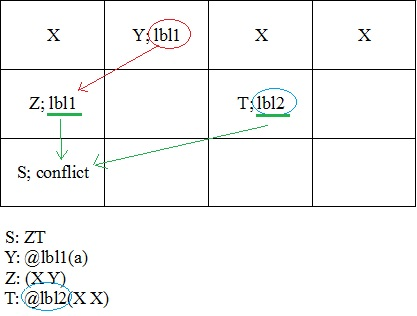
\includegraphics[width= 0.4\textwidth, height=0.4\textheight]{diagrams/table.png}}
    \end{center}
\end{frame}    

\begin{frame}
	\transwipe[direction=90]
	\frametitle{Результаты}
	\begin{itemize}
        \item Реализован алгоритм
        	\begin{itemize}
        	    \item определяет принадлежность диалекту
        	    \item печатает координаты характерных конструкций
    	    \end{itemize}
            \item Поставлен ряд экспериментов по определеню диалектов
        	\begin{itemize}
                \item Однозначно определён
                \item Конфликт
                \item Не удалось определить
            \end{itemize}
    \end{itemize}
\end{frame}    


\author[Ильнур Байгильдин]{}

\begin{frame}
	\transwipe[direction=90]
	\frametitle{Задача}
	\begin{itemize}
	    \item Интеграция алгоритма CYK, модифицированного, для работы с диалектами, с YaccConstructor
    	\begin{itemize}
            \item Расширение языка YARD возможностью использования меток в грамматике
            \item Реализация преобразования входной грамматики в эквивалентную ей грамматику в нормальной форме Хомского
        \end{itemize}
    \end{itemize}
\end{frame}

\begin{frame}[fragile]
	\transwipe[direction=90]
	\frametitle{Метки}
	Пример:
	\\
	\verb|s: X @name(a B c) S;|
	\\
	где @name - меткa, а в скобках находится последовательность характерных терминалов и нетерминалов.
\end{frame}

\begin{frame}
	\transwipe[direction=90]
	\frametitle{Преобразование грамматики}
	\begin{itemize}
	    \item Входная грамматика на языке YARD
	    \begin{itemize}
	        \item Содержит EBNF, метаправила
        \end{itemize}
        \item Необходимо преобразовать в CNF
        \begin{itemize}
            \item Преобразование в BNF
            \begin{itemize}
                \item существующие преобразования
                \item поддержка меток
            \end{itemize}
            \item Удаление $\varepsilon$-правил
            \item Удаление цепных правил
            \item Преобразование в CNF
        \end{itemize}
    \end{itemize}
\end{frame}    

\begin{frame}
	\transwipe[direction=90]
	\frametitle{Результаты}
	\begin{itemize}
        \item Грамматика поддерживает метки
        \item Добавлен алгоритм для преобразования грамматики в нормальную форму Хомского, с поддержкой меток
    \end{itemize}    
\end{frame}    

%%%%%%%%%%%%%%%%%%%%%%%%%%%%%%%%%%%%%%%%%%%%%%%%%%%%%%%%%%%%%%%%%%%%%%%%%%%%%%%%%%%%%%%%%%%%%%%%%%%%%%%
%%%    Использование GPGPU для синтаксичаского анализа
%%%%%%%%%%%%%%%%%%%%%%%%%%%%%%%%%%%%%%%%%%%%%%%%%%%%%%%%%%%%%%%%%%%%%%%%%%%%%%%%%%%%%%%%%%%%%%%%%%%%%%%

\author[Шенбин Илья]{}

\begin{frame}
	\transwipe[direction=90]
	\begin{block}{}
	    \begin{center}
	        \huge{Использование GPGPU для синтаксичаского анализа}
	    \end{center}
	\end{block}
	\begin{center}
	    \huge{Илья Шенбин}
	\end{center}
\end{frame}

\begin{frame}
	\transwipe[direction=90]
	\frametitle{Цель}
	Эффективная параллельная реализация алгоритма синтаксического анализа на GPU.
\end{frame}

\begin{frame}
	\transwipe[direction=90]
	\frametitle{Актуальность}
	\begin{itemize}
        \item Асимптотическая сложность парсеров КС-грамматик - $O(n^3)$, при этом размеры анализируемых строк огромны.
        \item Рост вычислительных мощностей процессоров за счёт увлечения числа ядер.
    \end{itemize}
\end{frame}    

\begin{frame}
	\transwipe[direction=90]
	\frametitle{Актуальность для проекта}
	\begin{itemize}
        \item Диалекты
        \item Быстрый синтаксический анализ
    \end{itemize}
\end{frame}

\begin{frame}
	\transwipe[direction=90]
	\frametitle{Задача}
	\begin{itemize}
        \item Изучение технологии CUDA
        \item Реализация:
    	\begin{itemize}
            \item Реализация CYK на языке С
            \item Распараллеливание алгоритма (по ячейкам в строке, по правилам...)
            \item Модификация и оптимизация алгоритма с учётом особенностей CUDA (оптимизация памяти, распределения потоков...)
        \end{itemize}

    \end{itemize}
\end{frame}    


\begin{frame}
	\transwipe[direction=90]
	\frametitle{Результаты}
	\begin{center}
        {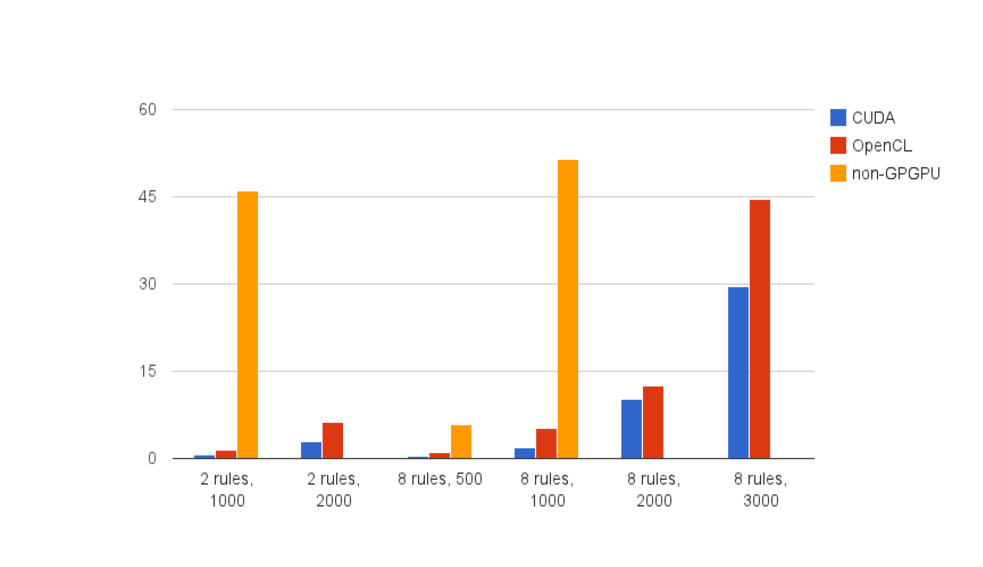
\includegraphics[width=\textwidth, height=0.9\textheight]{diagrams/CYKPerformance.pdf}}
    \end{center}
\end{frame}    

%%%%%%%%%%%%%%%%%%%%%%%%%%%%%%%%%%%%%%%%%%%%%%%%%%%%%%%%%%%%%%%%%%%%%%%%%%%%%%%%%%%%%%%%%%%%%%%%%%%%%%%
%%%    Интеграция YARD с Visual Studio
%%%%%%%%%%%%%%%%%%%%%%%%%%%%%%%%%%%%%%%%%%%%%%%%%%%%%%%%%%%%%%%%%%%%%%%%%%%%%%%%%%%%%%%%%%%%%%%%%%%%%%%

\author[Олег Щербаков, Артур Байков]{}

\begin{frame}
	\transwipe[direction=90]
	\begin{block}{}
	    \begin{center}
	        \huge{Интеграция YARD с Visual Studio}
	    \end{center}
	\end{block}
	\begin{center}
	    \huge
	        {Олег Щербаков
	        \\
            Артур Байков}
	\end{center}
\end{frame}

\begin{frame}
\frametitle{Цель}
    Реализация поддержки языка YARD в среде Visual Studio.
\end{frame}

\begin{frame}
	\transwipe[direction=90]
	\frametitle{Задача}
	\begin{itemize}
        \item Изучение F\#;
        \item Изучение и применение возможностей VS SDK;
        \item Реализация:
        	\begin{itemize}
            	\item перехода к определению;
            	\item подсветки вхождений выделенного нетерминала;
        	\end{itemize}
        \item Улучшение автодополнения.
    \end{itemize}
\end{frame}

\begin{frame}
	\transwipe[direction=90]
	\frametitle{Реализация}
	\begin{itemize}
        \item Обработка текста из активного окна;
        \item Обработка структуры solution и project в VS
        \item Модуль Data для работы с парсером и лексером языка YARD, а так же хранение промежуточных результатов и структуры проекта.
    \end{itemize}
    \begin{center}
        {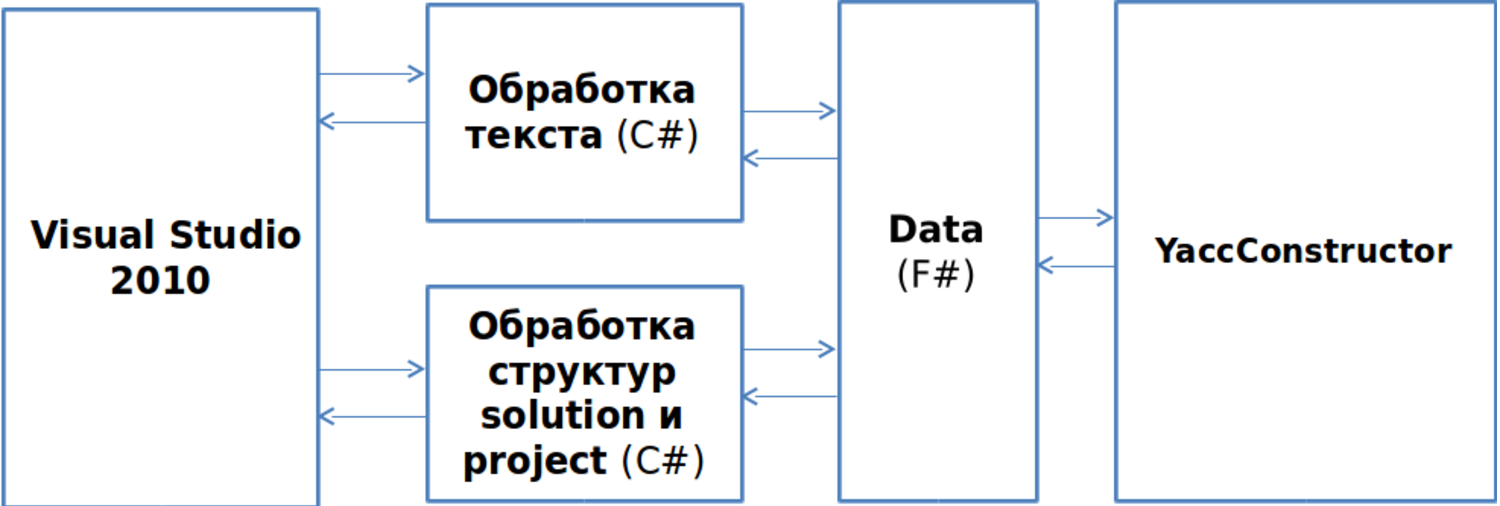
\includegraphics[width= 0.9\textwidth, height=0.4\textheight]{diagrams/VSYard1.pdf}}
    \end{center}
\end{frame}

\begin{frame}
	\transwipe[direction=90]
	\frametitle{Результаты}
	\begin{itemize}
        \item Реализованы:
	    \begin{itemize}
            \item переход к определению;
            \item подсветка вхождений выделенного нетерминала;
            
                
            	\begin{center}
                    {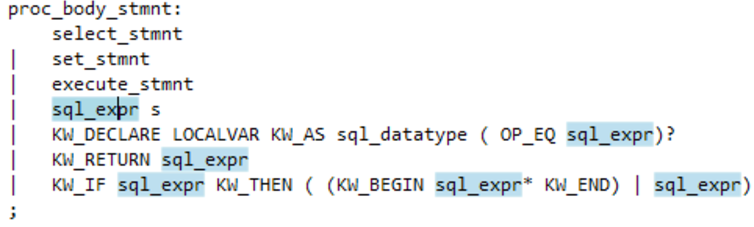
\includegraphics[width=0.4\textwidth, height=0.2\textheight]{diagrams/Select.pdf}}
                \end{center}
            
        \end{itemize}
        \item 
        {
            Улучшение автодополнения.
           	\begin{center}
                    {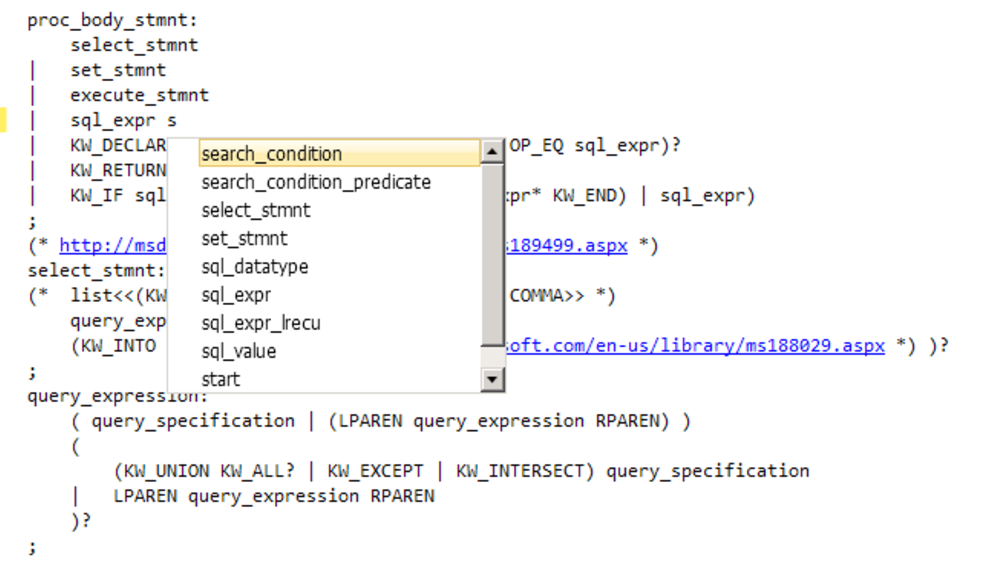
\includegraphics[width= 0.45\textwidth, height=0.35\textheight]{diagrams/Autocomplete.pdf}}
            \end{center}
        }
    \end{itemize}
\end{frame}
    
\author[Григорьев Семён]{}

\begin{frame}
	\transwipe[direction=90]
	\frametitle{Заключение}
	\begin{itemize}
        \item Сайт проекта: \href{http://recursive-ascent.googlecode.com} {http://recursive-ascent.googlecode.com}
	    \item Вопросы, пожелания, предложения:
	        \begin{itemize}
	            \item Semen.Grigorev@lanit-tercom.com
	            \item Ilia.Libis@lanit-tercom.com
            \end{itemize} 
    \end{itemize}
\end{frame}

\end{document}
